\documentclass[tikz,border=1pt]{standalone}
\usepackage{lmodern}\renewcommand{\familydefault}{\sfdefault}\usepackage[T1]{fontenc}\usepackage{amsmath,amssymb}
\usetikzlibrary{arrows.meta,positioning,calc}
\definecolor{ink}{HTML}{1A1A1A}\definecolor{gr}{HTML}{8A8A8A}\definecolor{grf}{HTML}{F2F2F2}
\definecolor{or}{HTML}{D55E00}\definecolor{orf}{HTML}{FDEEE6}\definecolor{gn}{HTML}{009E73}\definecolor{gnf}{HTML}{E6F5F0}
\definecolor{bl}{HTML}{0072B2}\definecolor{blf}{HTML}{E6F1F9}\definecolor{rd}{HTML}{C0392B}\definecolor{rdf}{HTML}{FBECEA}\definecolor{tn}{HTML}{8C7B6B}\definecolor{tnf}{HTML}{F1ECE6}
\tikzset{
  box/.style={draw=gr,fill=grf,line width=0.6pt,rounded corners=2pt,minimum height=0.8cm,align=center,inner sep=2pt,font=\footnotesize,text=ink},
  mukv/.style={box,draw=or,fill=orf,line width=0.8pt},
  blue/.style={box,draw=bl,fill=blf,line width=0.8pt},
  prior/.style={box,draw=tn,fill=tnf,line width=0.8pt},
  data/.style={-{Stealth[length=4pt,width=3.5pt]},line width=0.6pt,ink},
  flow/.style={-{Stealth[length=4pt,width=3.5pt]},line width=0.7pt,or},
  prio/.style={-{Stealth[length=4pt,width=3.5pt]},line width=0.7pt,tn,dashed},
  lab/.style={font=\scriptsize,inner sep=1pt,text=ink},
  head/.style={font=\bfseries\footnotesize,inner sep=1pt}
}
\newcommand{\bx}[2]{\textbf{#1}\\[-1pt]{\scriptsize #2}}
\begin{document}
\begin{tikzpicture}[x=1cm,y=1cm]
% ---- transformer layer, unmodified ----
\node[lab,text=gr,anchor=west] at (0.0,11.55) {transformer layer, unmodified};
\node[box,minimum width=1.3cm] (qkv) at (0.75,10.8) {\textbf{Q K V}};
\node[box,minimum width=3.0cm] (fa) at (3.2,10.8) {\bx{flash attention}{scores never stored}};
\node[box,minimum width=2.6cm] (out) at (6.9,10.8) {\textbf{layer output}};
\draw[data] (qkv) -- (fa); \draw[data] (fa) -- (out);
% ---- side node and measured heatmap ----
\node[mukv,minimum width=4.2cm] (kq) at (2.2,9.4) {\bx{kq\_evict side node}{softmax$(K\,Q^{\top}_{\text{last 16}})$, last chunk only}};
\draw[flow] (fa.south) -- (kq.north);
\node[inner sep=0,anchor=west] (heat) at (4.7,9.4) {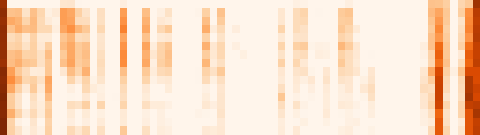
\includegraphics[width=3.4cm,height=0.8cm]{heat.pdf}};
\draw[or,line width=0.5pt] (heat.south west) rectangle (heat.north east);
\draw[flow] (kq.east) -- (heat.west);
\node[lab,anchor=south] at (heat.north) {$A\in\mathbb{R}^{16\times N}$, measured, log scale};
\node[blue,minimum width=4.6cm] (scores) at (4.2,8.0) {\bx{per-layer scores}{$s\in\mathbb{R}^{L\times N}$, reduced over the 16 queries}};
\draw[flow] (heat.south) -- ++(0,-0.35) -| (scores.north);
% ---- fork ----
\node[head,text=or,anchor=east] at (1.85,7.0) {(a) $\mu$KV};
\node[head,text=tn,anchor=west] at (6.7,7.0) {(b) per-head evictors};
\node[mukv,minimum width=3.9cm] (gate) at (2.05,6.15) {\bx{aggregate layers and heads}{one score per position, mean over $l,h$}};
\node[mukv,minimum width=3.9cm] (agg) at (2.05,5.2) {\bx{max-pool, kernel 7}{clusters survive, spikes do not}};
\node[mukv,minimum width=3.9cm] (alpha) at (2.05,4.25) {\bx{$\alpha$-gate}{$\alpha_a$ = distant mass, floor 0.70; split $K$}};
\node[blue,minimum width=3.9cm,minimum height=1.15cm] (keep) at (2.05,3.05) {\textbf{joint keep set, $K$ positions}\\[4pt]};
\draw[flow] (gate) -- (agg); \draw[flow] (agg) -- (alpha); \draw[flow] (alpha) -- (keep);
% keep-set strip proportional to the measured 4 / 721 / 299 split
\fill[bl!35!white,draw=bl,line width=0.4pt] (0.35,2.72) rectangle (0.37,2.97);
\fill[bl!55!white,draw=bl,line width=0.4pt] (0.37,2.72) rectangle (2.77,2.97);
\fill[blf,draw=bl,line width=0.4pt] (2.77,2.72) rectangle (3.75,2.97);
\node[lab,anchor=west] at (0.28,2.57) {sink 4}; \node[lab] at (1.75,2.57) {anchor 721}; \node[lab,anchor=east] at (3.85,2.57) {recent 299};
\node[prior,minimum width=3.9cm,minimum height=1.0cm] (ph) at (6.5,5.2) {\bx{per-head top-$K$}{each head keeps its own $K$ positions}};
\draw[flow] (scores.south) -- ++(0,-0.3) -| (gate.north);
\draw[prio] (scores.south) ++(0,-0.3) -| (ph.north);
\draw[prio] (ph) -- (6.5,2.25);
% ---- outcome panels ----
\fill[gnf,draw=gn,rounded corners=2pt,line width=0.8pt] (0.05,-0.1) rectangle (4.05,2.25);
\fill[rdf,draw=rd,rounded corners=2pt,line width=0.8pt] (4.5,-0.1) rectangle (8.5,2.25);
\node[head,anchor=north] at (2.05,2.2) {seq-level evict and compact};
\node[head,anchor=north] at (6.5,2.2) {union across heads};
\draw[flow] (keep.south) -- (2.05,2.25);
\fill[gn] (0.450,1.600) rectangle (0.640,1.750);
\draw[gn,densely dotted,line width=0.3pt] (0.675,1.600) rectangle (0.865,1.750);
\fill[gn] (0.900,1.600) rectangle (1.090,1.750);
\draw[gn,densely dotted,line width=0.3pt] (1.125,1.600) rectangle (1.315,1.750);
\draw[gn,densely dotted,line width=0.3pt] (1.350,1.600) rectangle (1.540,1.750);
\draw[gn,densely dotted,line width=0.3pt] (1.575,1.600) rectangle (1.765,1.750);
\draw[gn,densely dotted,line width=0.3pt] (1.800,1.600) rectangle (1.990,1.750);
\draw[gn,densely dotted,line width=0.3pt] (2.025,1.600) rectangle (2.215,1.750);
\draw[gn,densely dotted,line width=0.3pt] (2.250,1.600) rectangle (2.440,1.750);
\draw[gn,densely dotted,line width=0.3pt] (2.475,1.600) rectangle (2.665,1.750);
\fill[gn] (2.700,1.600) rectangle (2.890,1.750);
\fill[gn] (2.925,1.600) rectangle (3.115,1.750);
\draw[gn,densely dotted,line width=0.3pt] (3.150,1.600) rectangle (3.340,1.750);
\draw[gn,densely dotted,line width=0.3pt] (3.375,1.600) rectangle (3.565,1.750);
\fill[gn] (3.600,1.600) rectangle (3.790,1.750);
\fill[gn] (3.825,1.600) rectangle (4.015,1.750);
\fill[gn] (0.450,1.415) rectangle (0.640,1.565);
\draw[gn,densely dotted,line width=0.3pt] (0.675,1.415) rectangle (0.865,1.565);
\fill[gn] (0.900,1.415) rectangle (1.090,1.565);
\draw[gn,densely dotted,line width=0.3pt] (1.125,1.415) rectangle (1.315,1.565);
\draw[gn,densely dotted,line width=0.3pt] (1.350,1.415) rectangle (1.540,1.565);
\draw[gn,densely dotted,line width=0.3pt] (1.575,1.415) rectangle (1.765,1.565);
\draw[gn,densely dotted,line width=0.3pt] (1.800,1.415) rectangle (1.990,1.565);
\draw[gn,densely dotted,line width=0.3pt] (2.025,1.415) rectangle (2.215,1.565);
\draw[gn,densely dotted,line width=0.3pt] (2.250,1.415) rectangle (2.440,1.565);
\draw[gn,densely dotted,line width=0.3pt] (2.475,1.415) rectangle (2.665,1.565);
\fill[gn] (2.700,1.415) rectangle (2.890,1.565);
\fill[gn] (2.925,1.415) rectangle (3.115,1.565);
\draw[gn,densely dotted,line width=0.3pt] (3.150,1.415) rectangle (3.340,1.565);
\draw[gn,densely dotted,line width=0.3pt] (3.375,1.415) rectangle (3.565,1.565);
\fill[gn] (3.600,1.415) rectangle (3.790,1.565);
\fill[gn] (3.825,1.415) rectangle (4.015,1.565);
\fill[gn] (0.450,1.230) rectangle (0.640,1.380);
\draw[gn,densely dotted,line width=0.3pt] (0.675,1.230) rectangle (0.865,1.380);
\fill[gn] (0.900,1.230) rectangle (1.090,1.380);
\draw[gn,densely dotted,line width=0.3pt] (1.125,1.230) rectangle (1.315,1.380);
\draw[gn,densely dotted,line width=0.3pt] (1.350,1.230) rectangle (1.540,1.380);
\draw[gn,densely dotted,line width=0.3pt] (1.575,1.230) rectangle (1.765,1.380);
\draw[gn,densely dotted,line width=0.3pt] (1.800,1.230) rectangle (1.990,1.380);
\draw[gn,densely dotted,line width=0.3pt] (2.025,1.230) rectangle (2.215,1.380);
\draw[gn,densely dotted,line width=0.3pt] (2.250,1.230) rectangle (2.440,1.380);
\draw[gn,densely dotted,line width=0.3pt] (2.475,1.230) rectangle (2.665,1.380);
\fill[gn] (2.700,1.230) rectangle (2.890,1.380);
\fill[gn] (2.925,1.230) rectangle (3.115,1.380);
\draw[gn,densely dotted,line width=0.3pt] (3.150,1.230) rectangle (3.340,1.380);
\draw[gn,densely dotted,line width=0.3pt] (3.375,1.230) rectangle (3.565,1.380);
\fill[gn] (3.600,1.230) rectangle (3.790,1.380);
\fill[gn] (3.825,1.230) rectangle (4.015,1.380);
\fill[gn] (0.450,1.045) rectangle (0.640,1.195);
\draw[gn,densely dotted,line width=0.3pt] (0.675,1.045) rectangle (0.865,1.195);
\fill[gn] (0.900,1.045) rectangle (1.090,1.195);
\draw[gn,densely dotted,line width=0.3pt] (1.125,1.045) rectangle (1.315,1.195);
\draw[gn,densely dotted,line width=0.3pt] (1.350,1.045) rectangle (1.540,1.195);
\draw[gn,densely dotted,line width=0.3pt] (1.575,1.045) rectangle (1.765,1.195);
\draw[gn,densely dotted,line width=0.3pt] (1.800,1.045) rectangle (1.990,1.195);
\draw[gn,densely dotted,line width=0.3pt] (2.025,1.045) rectangle (2.215,1.195);
\draw[gn,densely dotted,line width=0.3pt] (2.250,1.045) rectangle (2.440,1.195);
\draw[gn,densely dotted,line width=0.3pt] (2.475,1.045) rectangle (2.665,1.195);
\fill[gn] (2.700,1.045) rectangle (2.890,1.195);
\fill[gn] (2.925,1.045) rectangle (3.115,1.195);
\draw[gn,densely dotted,line width=0.3pt] (3.150,1.045) rectangle (3.340,1.195);
\draw[gn,densely dotted,line width=0.3pt] (3.375,1.045) rectangle (3.565,1.195);
\fill[gn] (3.600,1.045) rectangle (3.790,1.195);
\fill[gn] (3.825,1.045) rectangle (4.015,1.195);
\fill[rd] (4.720,1.600) rectangle (4.910,1.750);
\fill[rd] (4.945,1.600) rectangle (5.135,1.750);
\fill[rd] (5.170,1.600) rectangle (5.360,1.750);
\draw[rd,densely dotted,line width=0.3pt] (5.395,1.600) rectangle (5.585,1.750);
\fill[rd] (5.620,1.600) rectangle (5.810,1.750);
\draw[rd,densely dotted,line width=0.3pt] (5.845,1.600) rectangle (6.035,1.750);
\draw[rd,densely dotted,line width=0.3pt] (6.070,1.600) rectangle (6.260,1.750);
\draw[rd,densely dotted,line width=0.3pt] (6.295,1.600) rectangle (6.485,1.750);
\draw[rd,densely dotted,line width=0.3pt] (6.520,1.600) rectangle (6.710,1.750);
\draw[rd,densely dotted,line width=0.3pt] (6.745,1.600) rectangle (6.935,1.750);
\draw[rd,densely dotted,line width=0.3pt] (6.970,1.600) rectangle (7.160,1.750);
\draw[rd,densely dotted,line width=0.3pt] (7.195,1.600) rectangle (7.385,1.750);
\draw[rd,densely dotted,line width=0.3pt] (7.420,1.600) rectangle (7.610,1.750);
\draw[rd,densely dotted,line width=0.3pt] (7.645,1.600) rectangle (7.835,1.750);
\fill[rd] (7.870,1.600) rectangle (8.060,1.750);
\fill[rd] (8.095,1.600) rectangle (8.285,1.750);
\fill[rd] (4.720,1.415) rectangle (4.910,1.565);
\draw[rd,densely dotted,line width=0.3pt] (4.945,1.415) rectangle (5.135,1.565);
\fill[rd] (5.170,1.415) rectangle (5.360,1.565);
\draw[rd,densely dotted,line width=0.3pt] (5.395,1.415) rectangle (5.585,1.565);
\draw[rd,densely dotted,line width=0.3pt] (5.620,1.415) rectangle (5.810,1.565);
\draw[rd,densely dotted,line width=0.3pt] (5.845,1.415) rectangle (6.035,1.565);
\draw[rd,densely dotted,line width=0.3pt] (6.070,1.415) rectangle (6.260,1.565);
\draw[rd,densely dotted,line width=0.3pt] (6.295,1.415) rectangle (6.485,1.565);
\draw[rd,densely dotted,line width=0.3pt] (6.520,1.415) rectangle (6.710,1.565);
\draw[rd,densely dotted,line width=0.3pt] (6.745,1.415) rectangle (6.935,1.565);
\fill[rd] (6.970,1.415) rectangle (7.160,1.565);
\fill[rd] (7.195,1.415) rectangle (7.385,1.565);
\draw[rd,densely dotted,line width=0.3pt] (7.420,1.415) rectangle (7.610,1.565);
\draw[rd,densely dotted,line width=0.3pt] (7.645,1.415) rectangle (7.835,1.565);
\fill[rd] (7.870,1.415) rectangle (8.060,1.565);
\fill[rd] (8.095,1.415) rectangle (8.285,1.565);
\fill[rd] (4.720,1.230) rectangle (4.910,1.380);
\draw[rd,densely dotted,line width=0.3pt] (4.945,1.230) rectangle (5.135,1.380);
\draw[rd,densely dotted,line width=0.3pt] (5.170,1.230) rectangle (5.360,1.380);
\draw[rd,densely dotted,line width=0.3pt] (5.395,1.230) rectangle (5.585,1.380);
\draw[rd,densely dotted,line width=0.3pt] (5.620,1.230) rectangle (5.810,1.380);
\draw[rd,densely dotted,line width=0.3pt] (5.845,1.230) rectangle (6.035,1.380);
\draw[rd,densely dotted,line width=0.3pt] (6.070,1.230) rectangle (6.260,1.380);
\draw[rd,densely dotted,line width=0.3pt] (6.295,1.230) rectangle (6.485,1.380);
\draw[rd,densely dotted,line width=0.3pt] (6.520,1.230) rectangle (6.710,1.380);
\fill[rd] (6.745,1.230) rectangle (6.935,1.380);
\fill[rd] (6.970,1.230) rectangle (7.160,1.380);
\draw[rd,densely dotted,line width=0.3pt] (7.195,1.230) rectangle (7.385,1.380);
\draw[rd,densely dotted,line width=0.3pt] (7.420,1.230) rectangle (7.610,1.380);
\fill[rd] (7.645,1.230) rectangle (7.835,1.380);
\fill[rd] (7.870,1.230) rectangle (8.060,1.380);
\fill[rd] (8.095,1.230) rectangle (8.285,1.380);
\fill[rd] (4.720,1.045) rectangle (4.910,1.195);
\fill[rd] (4.945,1.045) rectangle (5.135,1.195);
\fill[rd] (5.170,1.045) rectangle (5.360,1.195);
\draw[rd,densely dotted,line width=0.3pt] (5.395,1.045) rectangle (5.585,1.195);
\draw[rd,densely dotted,line width=0.3pt] (5.620,1.045) rectangle (5.810,1.195);
\draw[rd,densely dotted,line width=0.3pt] (5.845,1.045) rectangle (6.035,1.195);
\draw[rd,densely dotted,line width=0.3pt] (6.070,1.045) rectangle (6.260,1.195);
\draw[rd,densely dotted,line width=0.3pt] (6.295,1.045) rectangle (6.485,1.195);
\draw[rd,densely dotted,line width=0.3pt] (6.520,1.045) rectangle (6.710,1.195);
\draw[rd,densely dotted,line width=0.3pt] (6.745,1.045) rectangle (6.935,1.195);
\draw[rd,densely dotted,line width=0.3pt] (6.970,1.045) rectangle (7.160,1.195);
\fill[rd] (7.195,1.045) rectangle (7.385,1.195);
\draw[rd,densely dotted,line width=0.3pt] (7.420,1.045) rectangle (7.610,1.195);
\draw[rd,densely dotted,line width=0.3pt] (7.645,1.045) rectangle (7.835,1.195);
\fill[rd] (7.870,1.045) rectangle (8.060,1.195);
\fill[rd] (8.095,1.045) rectangle (8.285,1.195);
\fill[rd] (4.720,0.620) rectangle (4.910,0.770);
\fill[rd] (4.945,0.620) rectangle (5.135,0.770);
\fill[rd] (5.170,0.620) rectangle (5.360,0.770);
\fill[rd] (5.395,0.620) rectangle (5.585,0.770);
\fill[rd] (5.620,0.620) rectangle (5.810,0.770);
\draw[rd,densely dotted,line width=0.3pt] (5.845,0.620) rectangle (6.035,0.770);
\fill[rd] (6.070,0.620) rectangle (6.260,0.770);
\fill[rd] (6.295,0.620) rectangle (6.485,0.770);
\draw[rd,densely dotted,line width=0.3pt] (6.520,0.620) rectangle (6.710,0.770);
\fill[rd] (6.745,0.620) rectangle (6.935,0.770);
\fill[rd] (6.970,0.620) rectangle (7.160,0.770);
\fill[rd] (7.195,0.620) rectangle (7.385,0.770);
\draw[rd,densely dotted,line width=0.3pt] (7.420,0.620) rectangle (7.610,0.770);
\fill[rd] (7.645,0.620) rectangle (7.835,0.770);
\fill[rd] (7.870,0.620) rectangle (8.060,0.770);
\fill[rd] (8.095,0.620) rectangle (8.285,0.770);
\fill[gn] (0.450,0.620) rectangle (0.640,0.770);
\draw[gn,densely dotted,line width=0.3pt] (0.675,0.620) rectangle (0.865,0.770);
\fill[gn] (0.900,0.620) rectangle (1.090,0.770);
\draw[gn,densely dotted,line width=0.3pt] (1.125,0.620) rectangle (1.315,0.770);
\draw[gn,densely dotted,line width=0.3pt] (1.350,0.620) rectangle (1.540,0.770);
\draw[gn,densely dotted,line width=0.3pt] (1.575,0.620) rectangle (1.765,0.770);
\draw[gn,densely dotted,line width=0.3pt] (1.800,0.620) rectangle (1.990,0.770);
\draw[gn,densely dotted,line width=0.3pt] (2.025,0.620) rectangle (2.215,0.770);
\draw[gn,densely dotted,line width=0.3pt] (2.250,0.620) rectangle (2.440,0.770);
\draw[gn,densely dotted,line width=0.3pt] (2.475,0.620) rectangle (2.665,0.770);
\fill[gn] (2.700,0.620) rectangle (2.890,0.770);
\fill[gn] (2.925,0.620) rectangle (3.115,0.770);
\draw[gn,densely dotted,line width=0.3pt] (3.150,0.620) rectangle (3.340,0.770);
\draw[gn,densely dotted,line width=0.3pt] (3.375,0.620) rectangle (3.565,0.770);
\fill[gn] (3.600,0.620) rectangle (3.790,0.770);
\fill[gn] (3.825,0.620) rectangle (4.015,0.770);
\fill[gn] (3.000,0.620) rectangle (3.170,0.770);
\fill[gn] (3.200,0.620) rectangle (3.370,0.770);
\fill[gn] (3.400,0.620) rectangle (3.570,0.770);
\fill[gn] (3.600,0.620) rectangle (3.770,0.770);
\fill[gn] (3.800,0.620) rectangle (3.970,0.770);
\fill[gn] (4.000,0.620) rectangle (4.170,0.770);
\node[lab,rotate=90] at (0.25,1.35) {layers};
\node[lab,rotate=-90] at (8.38,1.35) {heads};
\node[lab] at (2.05,0.93) {token position}; \node[lab] at (6.5,0.93) {token position};
\node[lab] at (2.75,0.7) {$\to$}; \node[lab,anchor=north] at (6.5,0.55) {13 of 16 bins live};
\node[lab,text=gn,anchor=north] at (2.05,0.45) {same positions in every layer};
\node[lab,text=rd,anchor=north] at (6.5,0.25) {any head keeps it, it survives};
\node[lab,font=\bfseries\scriptsize,text=gn] at (2.05,-0.35) {live $=K$, contiguous};
\node[lab,font=\bfseries\scriptsize,text=rd] at (6.5,-0.35) {live $\gg K$, cannot compact};
\end{tikzpicture}
\end{document}
